{\documentclass [10pt,a4paper]{book}
\usepackage{graphicx}
\begin{document}
\begin{flushleft}
\textbf{80} CHAPTER SIX
\end{flushleft} 
\begin{flushleft}
\textbf{COMMUNITERO}
\end{flushleft}	 
CommunityZero supplies centralized collaborative services that give individual users access to any number of "communities"—some of which could be the focus of an e-research project. Unlike SharePoint, all CommunityZero communities are located on a single, central Web server. Individuals enroll for free and are allowed to partici-pate in as many different communities as they wish to create or join. CommunityZero pros-ides a larger suite of services to members than SharePoint and serves as a cus-tomizable portal for team members. Figure 6.2 provides a screen shot of a Communi-tyZero site that promotes the services provided.


CommunityZero provides asynchronous, threaded discussions; a "contributions" area where members can provide annotated links to sites or resources on the Web; a notice board feature for short announcements; and a list feature for creating itemized lists such as "checklists" and "to do" lists. CommunityZero provides real-time chat rooms and a series of "newsfeeds" from press agencies and other news organizations for team members. Like SharePoint, CommunityZero provides space for uploading and retrieving documents created by team members, but does not provide the notifi-cation services available in SharePoint that alert members when items change. 
\begin{center}
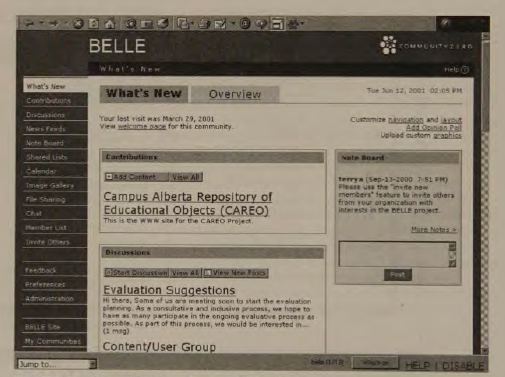
\includegraphics[scale=1]{2}
{FIGURE 6.2 Screen Shot from CommunityZero.TM}
\end{center}
\end{document}
 
